\subsection{Visualization of objects lists}

The published topics of \ac{GT} data and Camera-Calculation data are subscribed by \ac{ROS} node \textit{Object\_Visualization}. Each topic contains the ego-vehicle data and the specifically generated objects list. In \ac{RVIZ} the objects are represented by primitive figures with the help of marker messages. Figure \ref{fig:Nodes} shows the used topics and nodes. Rectangles represent topics and ellipses the called nodes. Moreover, tf is a package which controls the coordinate relationship of the ego-vehicle.
\begin{figure*}[thpb]
	\centering
	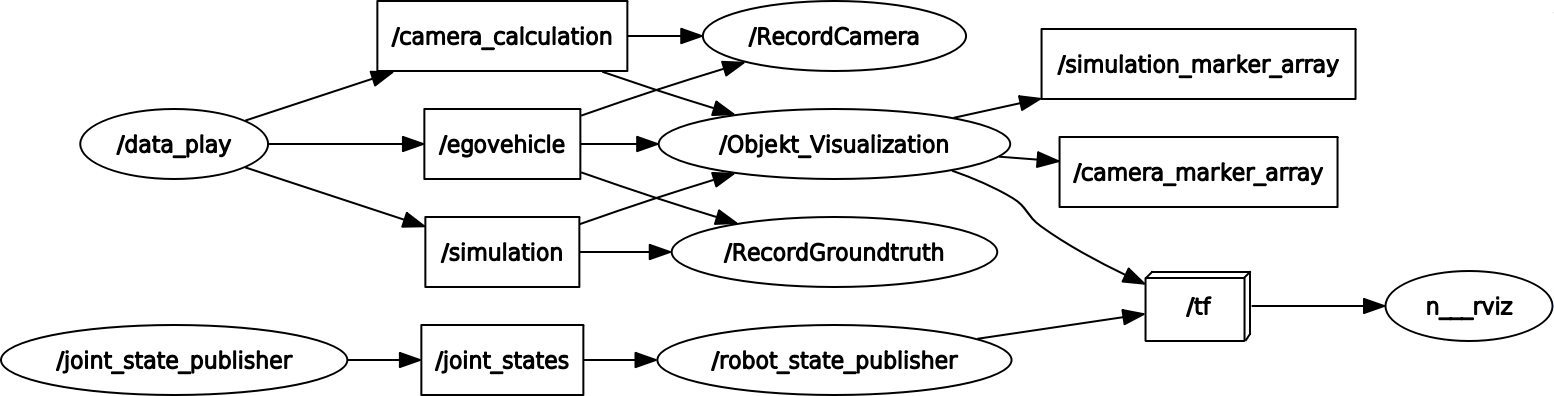
\includegraphics[width=0.85\linewidth]{rosgraph}
	\caption{Nodes (ellipses)/ Topics (rectangles) in \ac{ROS}}
	\label{fig:Nodes}
\end{figure*}
Marker messages are described with specific properties such as position, scale, type, color, orientation. Each object classification is assigned to one specific shape and color so that they can be differentiated in \ac{RVIZ}. The display variants for the possible object classes are shown in \cref{ClassificationAssignment}. 
\begin{table}[h]
	\caption{Classification Assignment}
	\begin{tabularx}{\columnwidth}{XXX}
		\toprule
		Classification & Shape & Color [RGB]\\
		\toprule
		car & cube & [1, 0, 0]\\
		truck & cube & [0, 1, 0]\\
		pedestrian & cylinder & [0, 0, 1]\\
		motorcyle & cube & [1, 0, 1]\\
		bicycle & cylinder & [1, 1, 0]\\
		stacionary & sphere & [0, 1, 1]\\
		other & sphere & [1, 1, 1]\\
		\bottomrule
	\end{tabularx}
	\label{ClassificationAssignment}
\end{table}

In addition, the yaw angle of the objects has to be transformed into a quaternion for the visualization in \ac{RVIZ}. The RGB alpha value of all markers for the calculated camera data is set to 0.5 so that the difference between camera data and GT data is visually recognizable. 
The highest detection probability of an object indicates the classification so that the marker message properties can be set to the corresponding values of \cref{ClassificationAssignment}. Furthermore, each detection position is mirrored on the Y-axis, because the vehicle coordinate system does not match the \ac{RVIZ} coordinate system. Finally, the generated markers are combined into a marker array and published.
The ego-vehicle is described as URDF model according to \cite{URDF}.
Furthermore, the model can be moved and rotated in the \ac{RVIZ} coordinate system by tf messages. 
The published topics of \ac{GT} data, Camera-Calculation data and ego-vehicle data are also saved in a Rosbag file. Each file contains the published ego data and the corresponding objects lists. In the following, these files are used for post-processing.